\documentclass{article}
\usepackage{graphicx}
\usepackage{amsmath}
\usepackage{fontsize}
\usepackage{cite}
\usepackage{color}
\usepackage{enumitem}
\usepackage{natbib}
\usepackage{tabularx}
\usepackage{natbib}
\usepackage{ragged2e}
\usepackage{sidecap}
\usepackage{geometry}
\geometry{a4paper, top=3cm, bottom=3cm, left=3.5cm, right=3.5cm}

\renewcommand*\contentsname{Indice} %Comando per cambiare il titolo del tableofcontents
\renewcommand\refname{Bibliografia} %Comando per cambiare il titolo delle References

\title{\Huge\textbf{La dis-informazione}}
\author{\texttt{Alessandro Meloni 0001118676 GEPID}}
\date{09/12/2023}

\begin{document}
\begin{figure}
    \centering
    \includegraphics[width=0.8\linewidth]{Immagini/Unibo arms.png}
\end{figure}
    \maketitle
\centering\tableofcontents
\newpage \section{Introduzione}
\flushleft
\begin{justify}
    Questo articolo avrà la finalità di spiegare cosa si intende per disinformazione e le varie sfaccettature che questo concetto può assumere.
    Faremo in modo di dare chiarezza in quanto la disinformazione ha di per sè una finalità negativa e di sviamento da ciò che è corretto, ma anche la sua forma non sempre risulta essere compresa agli occhi dei lettori.\\
    Innanzitutto partiremo con una piccola descrizione della disinformazione; successivamente analizzeremo una survey effettuata da parte dell'UNESCO nel 2023 e pubblicata dal The Guardian come articolo nella loro pagina internet.\citep{TheGuardian}\\ Questo sarà seguito da una piccola analisi del caso italiano, così da poterci fare un'idea della tendenza di percezione di questo concetto da parte della popolazione, visto che nella survey dell'UNESCO non è compresa.\\
    Introdurremo anche il Digital Service Act dell'UE e i suoi contenuti in merito ai social media.
    Seguirà successivamente una comparazione con alcuni dati relativi alla presenza oggettiva di fake news, valutando l'impatto che può avere nella vita delle persone, così da capire se le loro percezioni poi coincidono con la frequenza oggettiva del fenomeno all'interno dei vari media.
    In conclusione, vedremo i risultati che ha dato questa ricerca e i dati a nostra disposizione, analizzando anche il report di WEARESOCIAL del 2022 (ultimo a disposizione), al fine di dare dei consigli su come riconoscere informazioni da dis-informazioni e creare una maggiore consapevolezza/sicurezza nell'utente medio, evitando che questo fenomeno possa davvero portare al fine per cui la notizia viene diffusa.
\end{justify}

\begin{center}
\section{Il fenomeno della disinformazione}
\end{center}

\begin{justify}
    La disinformazione è quel fenomeno che viene studiato prevalentemente nelle scienze della comunicazione, ma che può espandersi a tanti altri rami.
    L'etimologia del termine risale al 1980, per la prima volta venne utilizzato il termine russo \textit{dezinformatzija}, la quale si riferisce a ‘‘un'arma’’ che venne istituita dal KGB e che consisteva semplicemente nel creare un ufficio ad hoc finalizzato alla diffusione e gestione della disinformazione, come attività di intelligence.\citep{DisWiki}\\
    Quindi dalla creazione dell'ufficio iniziò a diffondersi questo termine andando a colpire tutti gli Stati mondiali, chi più e chi meno.
\end{justify}

\centering\subsection{Cos'è la disinformazione?}

\begin{justify}
    La disinformazione è un concetto molto ampio e bisogna subito mettere in chiaro il fatto che non si riferisca esclusivamente a intenzioni malevoli, di fatto, è giusto come definito dalla sociologa \texttt{Claire Wardle} suddividere questo concetto in tre ramificazioni, comprendendo:
\begin{itemize}
    \item Disinformazione: la diffusione di notizie false con lo scopo specifico di trarre in inganno e sviare singoli soggetti, organizzazioni di persone o popolazioni intere: molte volte con finalità strettamente collegate ad ambito politico, finanziario ed interessi egoistici.
    \item Misinformazione: questo termine viene preso dall'inglese \textit{misinformation} e indica un'informazione che di per sè è falsa, ma senza l'effettiva finalità di nuocere altri soggetti da parte di colui o coloro che la diffondono. Certe volte è collegata alla divulgazione di informazioni facenti parte di un contenuto più ampio, senza però sapere che esiste questo contenuto;
    \item Malinformazione: termine che si distacca dalla normale definizione di ‘‘notizia falsa’’, però è opportuno ricomprenderla perchè ha come contenuto una notizia vera, ma che viene diffusa senza specificare il contesto così da arrecare danno ad uno specifico soggetto o soggetti coinvolti nella notizia. \citep{wardle2018information}
\end{itemize}
\end{justify}

\newpage\centering\subsection{Analisi dati:}

\begin{justify}    
Come già accennato nell'introduzione analizzeremo precisamente una sezione della survey che è stata condotta da parte dell'UNESCO in collaborazione con IPSOS, i cui dati sono stati raccolti dal 22 Agosto al 25 Settembre 2023, pubblicati dal The Guardian in data 7 Novembre 2023. \citep{Unesco}\\
Il campione analizzato è formato da 500 soggetti per ogni Stato dei 16 coinvolti, per una totalità campionaria di 8000 soggetti (con una popolazione totale pari a \textit{2.579.400.000} persone).
Questi 16 Stati sono suddivisi sulla base del loro \textit{HDI} (indice di sviluppo umano) e ogni Stato è stato scelto in previsione delle elezioni del 2024 (infatti vediamo che non è presente l'Italia).
Come definito dall'UNESCO, la finalità è stata quella di visualizzare e analizzare dando voce ai cittadini, quanto e come viene percepito l'impatto della disinformazione durante la loro vita quotidiana. D'altro canto, molto importante è stata la decisione di fare questa survey prima delle elezioni, proprio per comprendere se in questi casi potrebbe essere avvertita una maggiore diffusione di questo fenomeno.
\end{justify}

\centering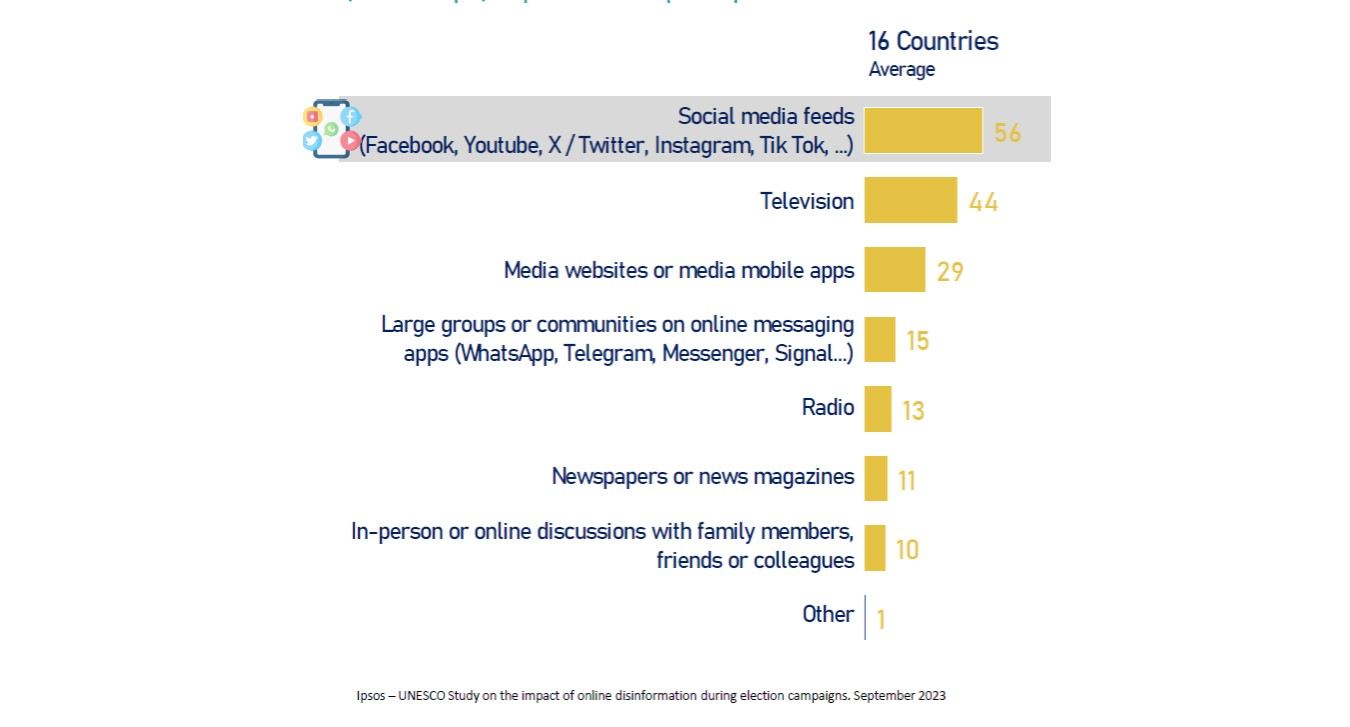
\includegraphics[width=0.6\linewidth]{Immagini/Grafico1.jpg}\\
    \begin{justify}
    Questo è il primo grafico realizzato sulla base della seguente domanda: \textit{‘‘Qual è lo strumento che utilizzi di più per reperire news e informazioni?’’}.
    In primis vediamo che gli strumenti che prevalgono sono i social network, con un distacco abbastanza sostanzioso dalla TV e altri media inseriti all'interno dello stesso grafico. Sicuramente questo sottolinea come prevalgano strumenti derivanti dall'avvento della digitalizzazione e dei social, poichè è molto più facile e veloce reperire le informazioni, visto che possono essere consultate in qualsiasi momento al contrario della TV, dove si dovrebbe andare al canale specifico e aspettare che facciano rivedere quel servizio.
    
\begin{center}
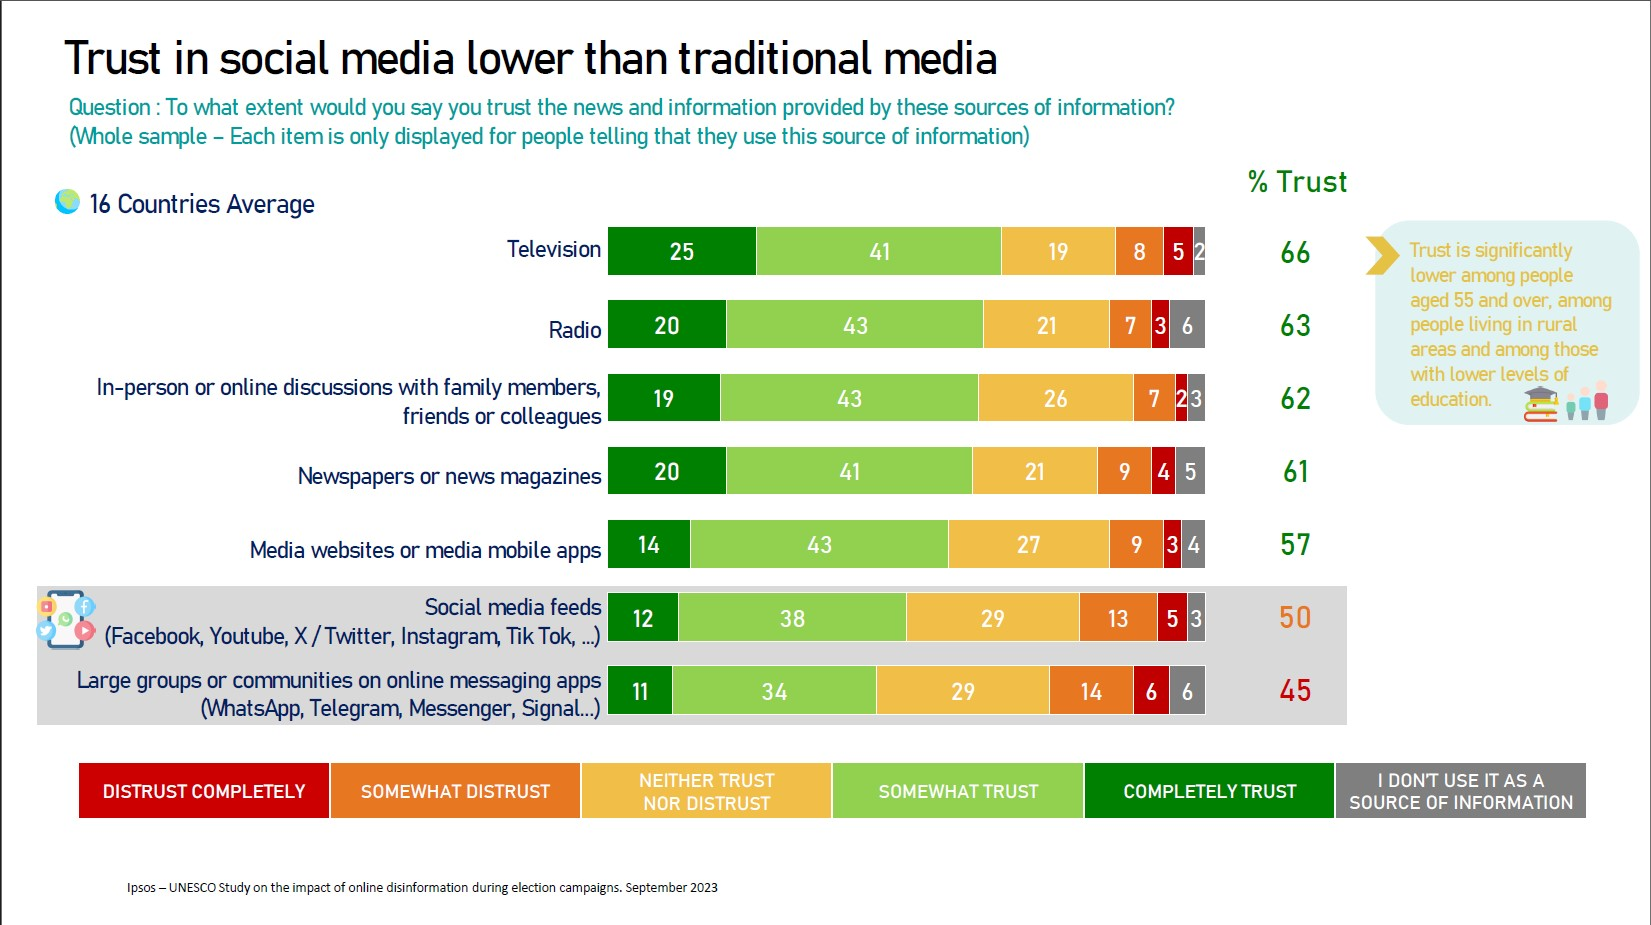
\includegraphics[width=0.6\linewidth]{Immagini/Grafico2.jpg}\\
\end{center}
    Oltre al fatto di capire come le persone si informano, bisogna comprendere anche il grado di fiducia che gli utenti affiancano a queste informazioni; invero, il secondo grafico rappresenta il grado di fiducia che le persone hanno rispetto ai media proposti nella prima domanda.
    Attraverso una scala nominale creata in riferimento alla domanda sottoposta è stato dato maggiore spazio di risposta agli intervistati (metodo che vedremo verrà confermato anche in alcuni dei prossimi grafici).
    Già da qua vediamo un controsenso, perchè gli intervistati si fidano di più dei media televisivi, radio, discussioni offline, giornali fisici e online, rispetto ai social media; mentre prima i social erano considerati come il mezzo prevalente nel reperire informazioni. A rigor di logica, quello che utilizzi di più dovrebbe coincidere anche con quello di cui ti fidi di più, invece in questo caso non accade. Potremmo intuire che i social vengano utilizzati più per finalità ricreative e ludiche: per questo si presenta questa contraddizione.
    
\begin{center}
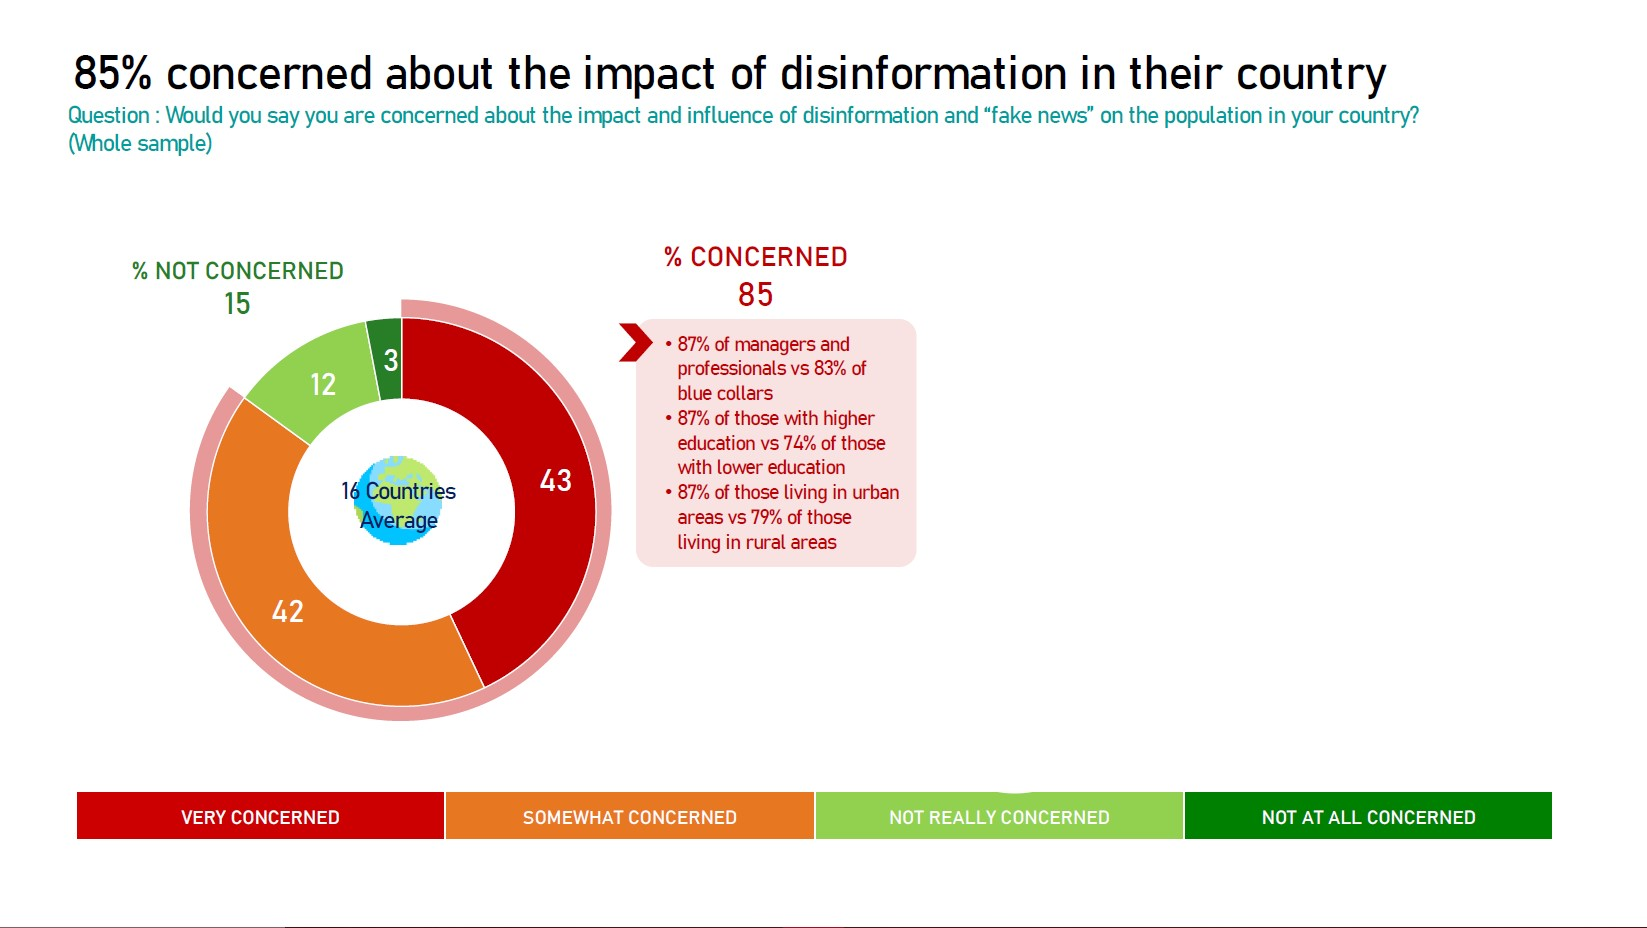
\includegraphics[width=0.6\linewidth]{Immagini/Grafico3.jpg}\\
\end{center}
    Ad ogni modo il terzo grafico segue la stessa linea logica, infatti viene chiesto quanto le persone siano preoccupate della disinformazione e delle fake news nel proprio paese.
    Il dato che subito balza all'occhio è la stragrande prevalenza degli utenti ‘‘molto preoccupati’’ (43\%) e ‘‘abbastanza preccupati’’ (42\%). Considerando la suddivisione dei gruppi è un risultato che dimostra ci sia una forte percezione negativa del fenomeno.

\begin{center}
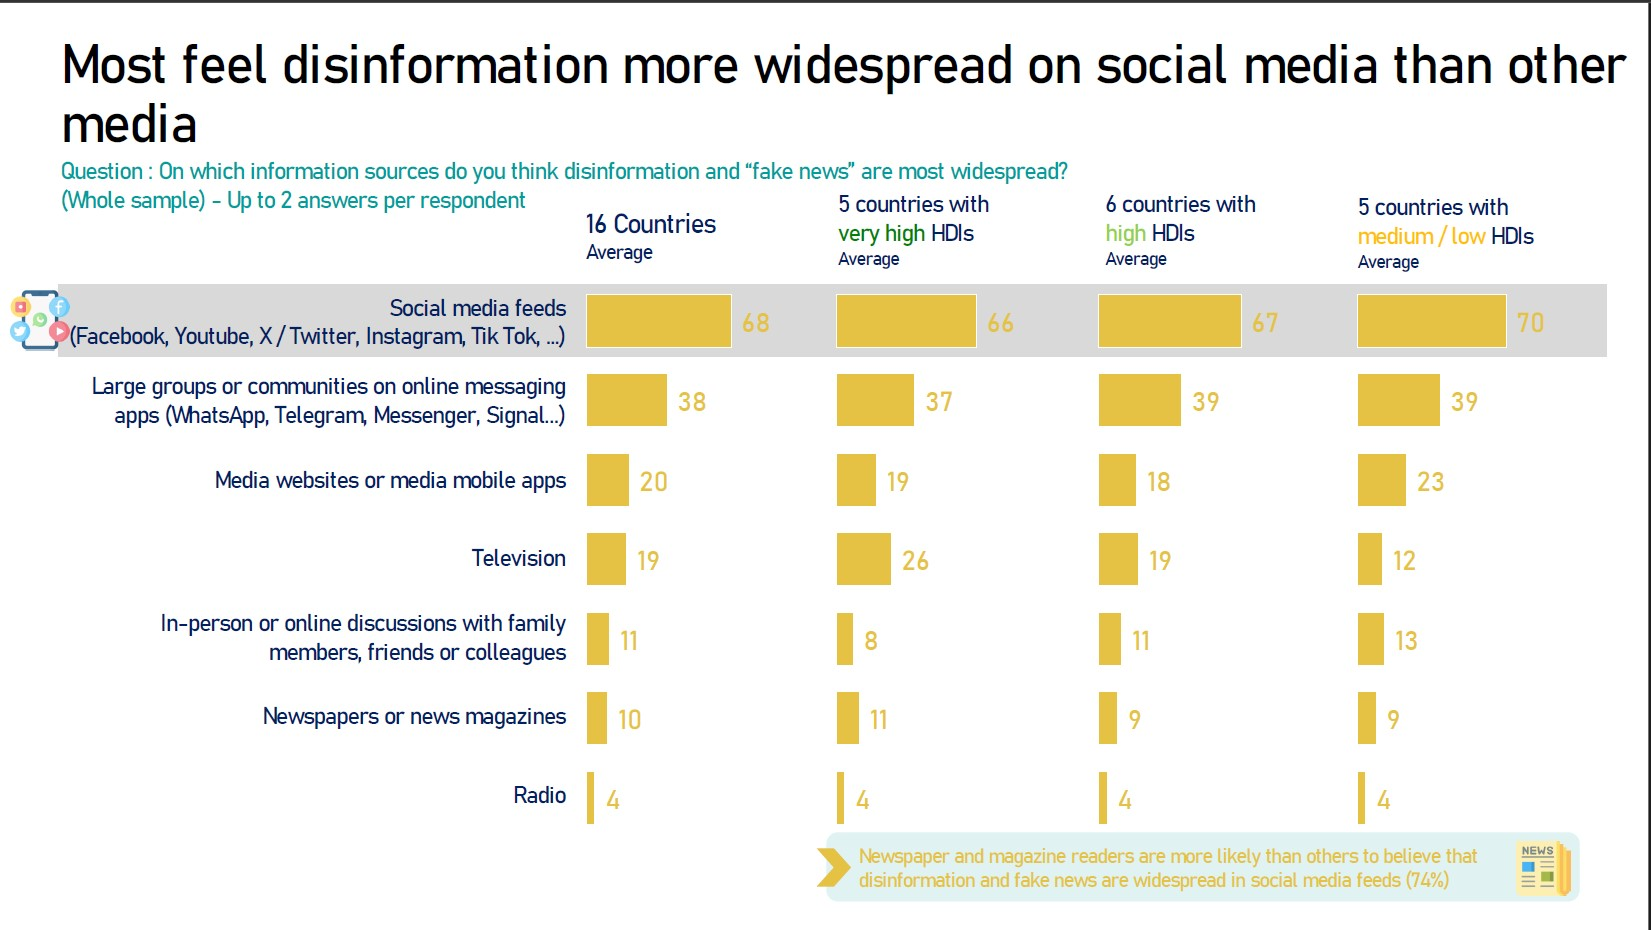
\includegraphics[width=0.6\linewidth]{Immagini/Grafico4.jpg}\\
\end{center}
    A questo punto bisogna comprendere dove gli utenti sentono che la disinformazione è più diffusa. Con l'ausilio del seguente grafico osserviamo che i social sono quelli che prevalgono, con una percentuale molto più alta anche solo dal secondo posto: evidenziando il trend dei grafici precedenti.\\
    Come già accennato all'inizio l'Italia non è presente all'interno del sondaggio, ma secondo il \textit{3° Rapporto Ital-Communication Censis}, circa il 83\% degli italiani utilizza il web per informarsi e il 74\% i media tradizionali: dunque, i dati seguono la falsariga di quelli intervistati dall'UNESCO.
    In più, circa il 76\% degli italiani pensa che l'individuazione delle fake news sia più complessa, anche a causa dello sviluppo di sistemi più sofisticati come le AI (lo pensa il 75\%); allo stesso modo c'è anche positività nell'utilizzo di questa tecnologia, con circa il 59\% che suppone possa garantire ulteriori strumenti per riuscire a contrastarle.\\
    Infine, in riferimento a questi ultimi dati, una percentuale pari al 20\% afferma di non avere le conoscenze per poterle distinguere.\citep{chiariello_disinformazione_2023}
\end{justify}

\centering\newpage\subsection{Digital Service Act e Social Media}
\begin{justify}
    Collegandoci a quanto e come viene percepita la disinformazione da parte dell'utente, vediamo che l'UE è intervenuta in quest'ambito con l'introduzione del \textit{Digital Service Act}: Regolamento UE 2065/2022.\\
    Questo regolamento ha portato a una rivoluzione normativa con ulteriori documenti e aggiornamenti di documenti già esistenti (il GDPR, la redazione dell'AI ACT e via discorrendo).
    Sulla base delle nuove regole inserite, dall'Aprile del 2023 sono diciannove le società poste sotto il controllo della Commissione UE: tra le più importanti Facebook, Twitter, TikTok, Instagram e Youtube.\citep{dariano_disinformazione_2023}\\
    Il 25 Agosto 2023 è stata la data stabilita come scadenza per adattarsi alle normative inserite nel regolamento, con la finalità di garantire nuove istanze di trasparenza e responsabilizzazione, favorendo informazioni pluralistiche ma al tempo stesso ‘‘non inquinate’’: è qua che si presenta il dato più allarmante per l'Italia. Secondo il primo codice di auto-disciplina (rapporto di valutazione dei rischi sistemici), presentato in riferimento al primo semestre all'UE da parte delle \textit{tech companies} sotto controllo, Meta, solo in Europa, ha rimosso 140.000 contenuti considerati \textit{‘‘dannosi per la salute, con interferenza elettorale o sui censimenti’’}, di cui 45.000 provengono solo da Facebook Italia: diventando il paese più esposto alle social \textit{fake news} in Europa (si aggiungono ulteriori 1900 contenuti da Instagram).\\
    Seguono poi la Germania al secondo posto con 22.000 contenuti e al terzo la Spagna con 16.000.
    Parallelamente, l'Italia è al secondo posto in Europa per contenuti verificati, circa 7 milioni, contro i 7.4 milioni della Francia che la portano al primo posto (essendosi piazzata al quinto posto per contenuti cancellati, ha un miglior rapporto con i contenuti verificati).
    Questo evidenzia l'impegno di Meta nelle verifiche, con il taglio dei contributi a canali che divulgano materiale falso, passando da 20 a 26 aziende di \textit{fact checking} (aziende che si occupano di controllo di informazioni) e dando a milioni di utenti la possibilità di disattivare alcuni contenuti personalizzati.\citep{tg24_fake_2023}\\
    X (ex Twitter) non è stato citato nei dati proprio perché inizialmente con la nuova proprietà targata Elon Musk prese posizione, non accettando la presentazione del codice di auto-disciplina e decidendo di adattarsi dal 25 di Agosto.\\
    Pur essendo considerata dall'UE come \textit{piattaforma con la maggior presenza di post con cattiva informazione o disinformazione}, ha introdotto una politica che vieta agli utenti di prendere di mira chiunque attui comportamenti legati all'\textit{hatespeech} (campagne/iniziative d'odio nei confronti di certe persone).
    Molto probabilmente le diatribe nascono perché conviene alle \textit{tech companies} lasciar diffondere questi fenomeni, giacchè, oltre a creare una maggiore propagazione del contenuto, porta anche più persone a discuterne e indipendentemente dal fatto che il contenuto sia positivo o negativo, una maggiore interazione e condivisione fa guadagnare di più le aziende.
\end{justify}

\centering
\newpage\section{Riflessioni e conclusioni}
\begin{justify}
    In conclusione, dati alla mano osserviamo che la situazione può avere un'interpretazione positiva o negativa, dipende tanto dai punti di vista che le persone sviluppano in riferimento a determinate tematiche. Possiamo affermare che le percezioni delle persone possono coincidere con la realtà, in questo caso la percezione negativa sulla disinformazione, almeno in Italia, si è rivelata vera, sulla base del rapporto da consegnare all'UE.\\
    Secondo la ricerca \textit{Digital 2023: Global Overview report} di WEARESOCIAL è emerso che tra gli utenti dai 16 ai 64 anni sono 5.44 miliardi le persone che hanno uno smartphone, 5.16 miliardi le persone che usano internet e 4.76 miliardi hanno un account nei social media. In aggiunta le persone utilizzano con una media giornaliera di 6 ore e 37 minuti internet, 3 ore e 23 minuti la tv (comprendendo anche broadcast e streaming che prendono gran parte delle ore di questo gruppo) e 2 ore e 31 minuti i social.\citep{WEARESOCIAL}\\
    Le persone passano più tempo davanti a dispositivi elettronici, in internet e nei social, ragion per cui potrebbe essere più probabile incappare in contenuti fuorvianti e in disinformazione. Questo se pensiamo che la correlazione tra tempo trascorso e contenuti di questo tipo possa essere positiva, ma, come mostra la ricerca di Vaccari e Valeriani, non tutto si presenta sempre come ci aspettiamo, pertanto, non avendo ricerche o dati che mettano in correlazione questi due aspetti, possiamo solo fare delle supposizioni sulla base dei dati di cui disponiamo fino ad ora.\citep{vaccari_outside_2021}\\
    Tuttavia rimane il problema nel riuscire a riconoscerle, sicchè i consigli che si possono dare sono:
    \begin{enumerate}
    \item Diversificare i propri mezzi di informazione, così da non polarizzarsi su certe idee ed avere un bagaglio di conoscenze più ampio, il quale potrebbe sicuramente aiutare a riconoscere buona informazione da cattiva informazione.
    \item Mai basarsi unicamente sul titolo dell'articolo, può capitare che siano titoli ingannevoli, dunque è sempre meglio leggere tutte le informazioni e poi fare un'opportuna valutazione.
    \item Infine mantenere o sviluppare un pensiero critico tale per cui ogni qualvolta si legga una notizia su internet (o in generale), la si metta in discussione e ci si informi in materia, senza sentenziare o affermare che ciò che si legge o il mezzo che si utilizza sia verità assoluta.
    \end{enumerate}
\end{justify}
\newpage
\begin{justify}
    \bibliography{Bibliografia}
    \bibliographystyle{plainnat}
\end{justify}
    
\end{document}